In questa sezione viene presentato il prospetto economico in cui vengono riportate le spese effettivamente sostenute. Si riportano le ore impiegate per svolgere le attività programmate, sia per ruolo che per membro del gruppo. In base alla differenza ottenuta tra preventivo e consuntivo, detta conguaglio, si avrà un bilancio:
\begin{itemize}
	\item \textbf{Positivo:} se il preventivo ha superato il consuntivo; 
	\item \textbf{Negativo:} se il consuntivo ha superato il preventivo;
	\item \textbf{In pari:} se consuntivo e preventivo coincidono.
\end{itemize}

\subsection{Analisi}
Si riporta di seguito il consuntivo della macro-fase di \textit{Analisi}.

\noindent La seguente tabella riporta la differenza di ore impiegate rispetto a quanto preventivato, divise per ruolo. I valori negativi nella tabella indicano un monte ore maggiore di quello preventivato, i valori positivi una diminuzione di ore.

\begin{table}[h]
\centering
\begin{tabular}{|l|c|c|}
	\toprule
	\textbf{Ruolo} & \textbf{Ore per ruolo} & \textbf{Costo per ruolo} \\
	
	\midrule
	Responsabile di Progetto & 1 & 30 \\
	Amministratore di Progetto & 1 & 20 \\ 
	Analista & -2 & -50 \\
	Progettista & & \\
	Programmatore & & \\
	Verificatore & -1 & -15 \\
	\midrule
	\textbf{Totale} & -1 & -15 \\
		
	\bottomrule
\end{tabular}
\caption{Differenza ore e costo per ruolo, Analisi}
\label{tab3}
\end{table} 

\noindent La seguente tabella riporta le differenze tra ore preventivate e quelle impiegate, per membro, durante la macro-fase di Analisi: 
\begin{table}[h]
\centering
\begin{tabular}{|l|c|c|c|c|c|c|c|}
	\toprule
	\textbf{Cognome e Nome} & \multicolumn{6}{c}{\textbf{Ore per ruolo}} & \textbf{Ore Totali} \\
	& \textbf{Re} & \textbf{Am} & \textbf{An} & \textbf{Pt} & \textbf{Pr} & \textbf{Ve} & \\
		
	\midrule
	Agostinetto Matteo & & & -1 & & & & -1 \\
	Burlin Valerio & 1 & & & & & & 1 \\ 
	Carraro Nicola & & & -1 & & & & \\
	Crespan Emanuele & & 1 & & & & & 1 \\
	Ros Fabio & & & & & & & \\
	Suierica Bogdan & & & & & & -1 & -1 \\
		
	\bottomrule
\end{tabular}
\caption{Differenza ore a componente per ruolo, Analisi}
\end{table}

\newpage
\noindent Il seguente grafico riporta la differenza tra le ore preventivate e quelle impiegate, per ruolo, durante la macro-fase di Analisi:
\begin{figure}[h]
\centering
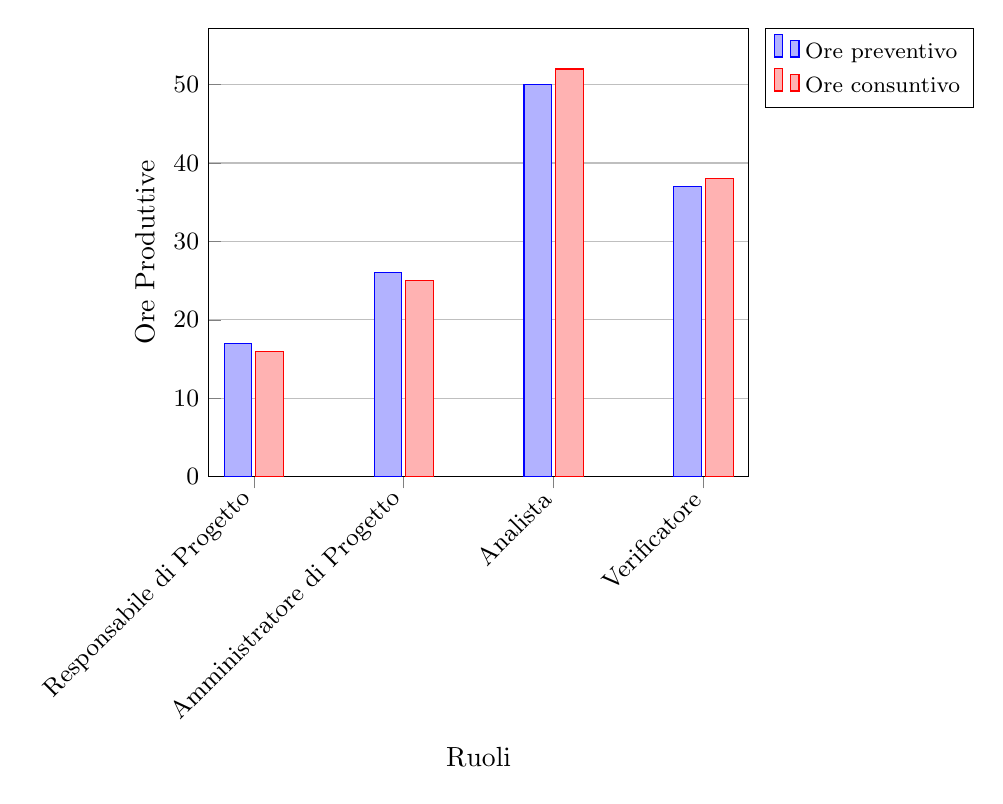
\begin{tikzpicture}
\begin{axis}[
	ybar,
	tick label style={font=\small},
	tickpos=left,
	xlabel = {Ruoli},
	ylabel = {Ore Produttive},
	xticklabels={Responsabile di Progetto, Amministratore di Progetto, Analista, Verificatore}, 
	xtick={1,2,3,4},
	x tick label style = {rotate=45,anchor=east},
	ymin=0,
	ymajorgrids = true,
	legend pos = outer north east,
	legend style = {nodes=right,font=\footnotesize},
]
\addplot +[bar shift=-.2cm] plot coordinates {(1, 17) (2, 26) (3, 50) (4, 37)};

\addplot +[bar shift=.2cm] plot coordinates {(1, 16) (2, 25) (3, 52) (4, 38)};
\legend{\strut Ore preventivo, \strut Ore consuntivo}
\end{axis}
\end{tikzpicture}
\caption{Differenza preventivo-consuntivo, Analisi}
\end{figure}

\subsubsection{Conclusioni}
Dalla tabella~\ref{tab3} si può notare come per svolgere le attività riportate nel diagramma di \gls{Gantt} in figura~\ref{fig1} è stata necessaria un'ora in più di quanto preventivato, con un aumento dei costi di \textbf{15 euro}. Tale passivo non andrà ad influire sul costo totale del progetto in quanto i costi sostenuti in questa macro-fase non vengono poste a carico del Proponente.  

